
\ifx\isEmbedded\undefined

%%%%% copy from main
\documentclass[twoside,openright,titlepage,a4paper,11pt,chapterprefix,appendixprefix]{scrreprt}%
%\usepackage[ngerman]{babel} % deutsche Silbentrennung
\usepackage[ansinew]{inputenc} % wegen deutschen Umlauten
\usepackage{graphicx}
\usepackage{subfigure}
\subfigcapmargin = 0.2cm
\usepackage{mathcomp}
\usepackage{amsmath}
\usepackage[format=plain ,margin={1cm,1cm}]{caption} %koma script ist standartm��ig auf "hang", links und rechts einger�ckt
\usepackage{chapterfolder}
% and we re-write includegraphics
\let\includegraphicsWithoutCF\includegraphics
\renewcommand{\includegraphics}[2][]{\includegraphicsWithoutCF[#1]{\cfcurrentfolder#2}}


\pagestyle{headings} % wir wollen auf jeder Seite eine Ueberschrift

\setlength{\unitlength}{1cm}
\setlength{\oddsidemargin}{0.3cm}
\setlength{\evensidemargin}{0.3cm}
\setlength{\textwidth}{15.5cm}
\setlength{\topmargin}{-0.7cm}
%\setlength{\textheight}{22cm} %bei seitlich
\setlength{\textheight}{23cm} %bei mittig
%%%%%%%%%%%%%%%%%%%%%%%%%%%%%%%%%%%%%%%%%%%%%%


\begin{document}


\else
\fi
% ******************************************************************************

\section{FED configuration}
\begin{itemize}
\item 1 CTA + 1 FITEL Rx FMC (in upper slot for current PixFED beta FW - in lower slot in the future)
\item Xilinx FMC105 supported on the other slot for debugging (\url{https://indico.cern.ch/event/482128/contribution/0/attachments/1211056/1766370/Phase_1_update_13_01_2016.pdf} for Pin mapping)
\item current FW is rather basic (phase finding, FE DESER block, basic BE readout functionality)
\begin{itemize}
\item single-event readout mode / TTS / C-DAQ implementation in progress
\item photocurrent measurement via ADC on FMC implemented
\item OSD read back functionality implemented
\end{itemize}
\item integration in POS ongoing - standalone CMD line tool available: \url{https://github.com/gauzinge/FED_burnin/tree/FIFO} - gcc > 4.7 required!!
\item caveat: uTCA FED needs male MPO on input fibre (different from digital VME FED)
\end{itemize}

\section{FED performance measurements}

Here we could collect some results and 'How-to's for the performance measurements for the FEDs


\begin{figure}[]
\centering
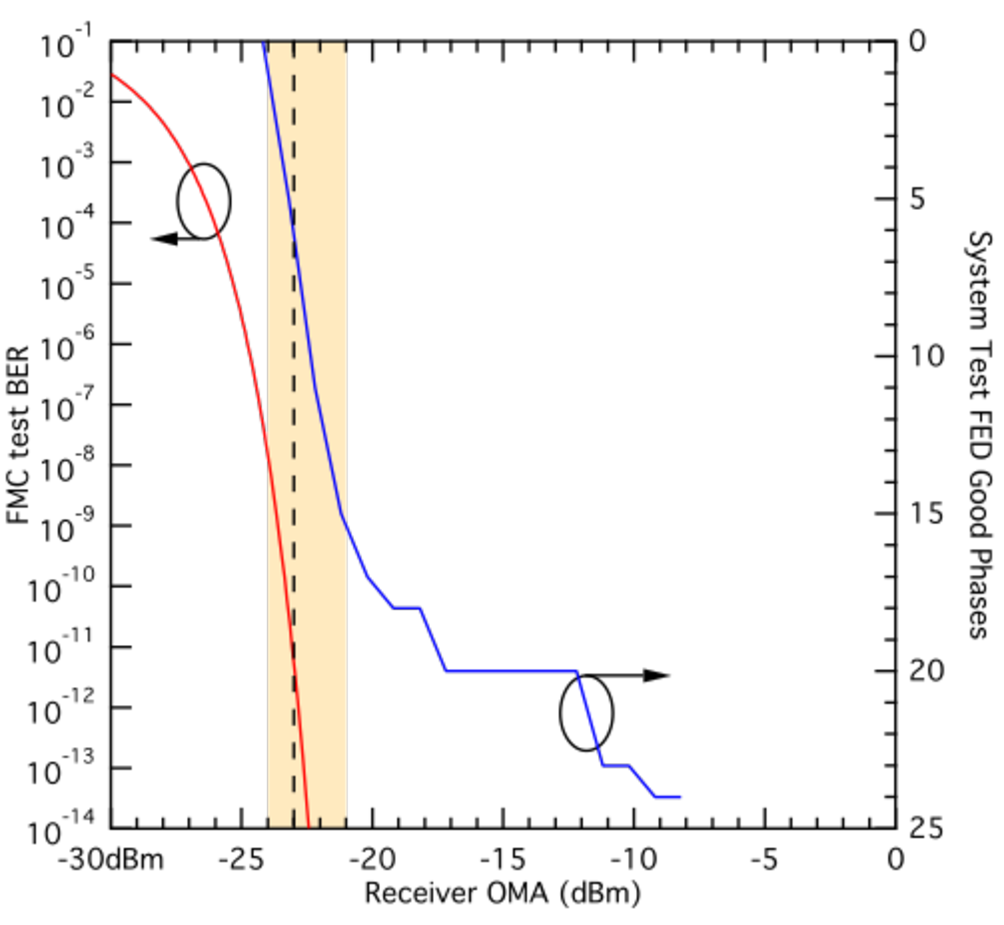
\includegraphics[width=\textwidth]{../images/GoodPhasesAttenuationTest.pdf}
\caption[Number of good phases vs optical signal attenuation]{\label{pic:GoodPhasesVsAttenuation} \textbf{Number of good phases vs optical signal attenuation}\\
}
\end{figure}



% ******************************************************************************
\ifx\isEmbedded\undefined
\input{../biblio.tex}
\end{document}
\else
\fi
